\documentclass[writeup.tex]{subfiles}
\begin{document}

			
	
\section{Quests} \label{section.quests}
	Here's a short walkthrough of each of the quests.

	\begin{figure}[H]
		\centering
		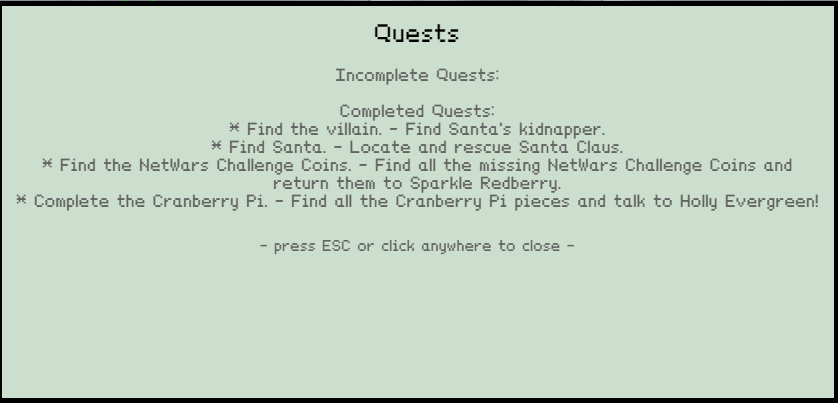
\includegraphics[width=.9\linewidth]{screenshots/quests}
		\caption{The in-game quest screen.}
	\end{figure}
	
	Now, to make it easier to find each of the items there is a little trick that can be done. When looking at the source of the HTML page with the game, you can find the following
	
	\begin{figure}[H]
		\centering
		\includegraphics[scale=1]{"screenshots/canvas html"}
	\end{figure}
	
	The canvas with id 'floating' is what renders the overlay of certain objects, such as the roofs and such. Now, since the site is using jQuery, it's quite easy to toggle the visibility of items, when they have an id. So open the developer console..
	
	\begin{figure}[H]
		\centering
		\includegraphics[scale=1]{"screenshots/coins"}
	\end{figure}
	
	Type in \lstinline!jQuery("#floating").toggle()! and it'll toggle the visibility. The reason to use toggle, is to make it easy to hit arrow up and hit enter, to toggle it again.

	\subsection{Find Santa} \label{subsection.quest_find_santa}
		So, to find Santa one needs to solve a few of the terminals, more specifically \autoref{terminal4} and \autoref{terminal5}. \textit{Now, to be honest, I'm not sure if you have to solve the rest of the terminals, but if you do, check out the solutions in \autoref{section.part3}}.\\
		\\
		Once those 2 terminals are solved you can go to 1978. Once there, head back up into the workshop and in through the door that belongs to \autoref{terminal4} and you will find Santa waiting for you.
	
	\subsection{Complete the Cranberry Pi} \label{subsection.quest_cranberry_pi}
		You get this quest when you speak with Holly Evergreen in The North Pole. She asks you to find all the pieces of a Cranberry Pi. Go to the locations shown in the following 5 figures, once you collected all the items, return to Holly Evergreen and she will give you the Cranberry Pi image, which is needed to complete Part 3\footnote{See \autoref{section.part3} to see how to complete this part.} of the story line.
		
		
		\begin{figure}[H]
			\centering
			\begin{minipage}{.5\textwidth}
				\centering
				\includegraphics[scale=1]{"screenshots/items/Cranberry Pi - Cranberry Pi Board"}
			\caption{Cranberry Pi Board\\Inside the Secret Fireplace Room in Elf House \#1.}
			\end{minipage}%
			\begin{minipage}{.5\textwidth}
				\centering
				\includegraphics[scale=1]{"screenshots/items/Cranberry Pi - HDMI Cable"}
				\caption{HDMI Cable\\Can be found in the Workshop.}
			\end{minipage}
		\end{figure}
		\begin{figure}[H]
			\centering
			\begin{minipage}{.5\textwidth}
				\centering
				\includegraphics[scale=1]{"screenshots/items/Cranberry Pi - Heat Sink"}
				\caption{Heat Sink\\Can be found in Elf House \#2 - Upstairs.}
			\end{minipage}%
			\begin{minipage}{.5\textwidth}
				\centering
				\includegraphics[scale=1]{"screenshots/items/Cranberry Pi - Power Cord"}
			\caption{Power Cord\\Is hidden behind the snowman outside.}
			\end{minipage}
		\end{figure}

		\begin{figure}[H]
			\centering
			\includegraphics[scale=1]{"screenshots/items/Cranberry Pi - SD Card"}
			\caption{SD Card\\Located on the small walkway to the left of the Workshop.}
		\end{figure}
		
		
	\subsection{Find the NetWars Challenge Coins} \label{subsection.quest_find_netcoins}
		So there are 20 coins to find in total. 13 in today's world and 7 in the year 1978. Some coins are only reachable once you complete terminals, so this means that to collect them all you need to solve most of the terminals. How to solve them can be found in \autoref{section.part5}. Once the terminals are completed, or while moving between them check out these locations.
		
		\subsubsection*{Today}
			All these coins are found in today's world.
			\begin{figure}[H]
				\centering
				\includegraphics[scale=1]{"screenshots/coins/Netcoin - Elf House 1 - Secret Fireplace Room"}
				\caption{Found inside the fireplace in Elf House \#1.}
			\end{figure}
			
			\begin{figure}[H]
				\centering
				\includegraphics[scale=1]{"screenshots/coins/Netcoin - Elf House 2 - On shelf"}
				\caption{Found inside Elf House \#2 on the shelfs}
			\end{figure}
			
			\begin{figure}[H]
				\centering
				\includegraphics[scale=1]{"screenshots/coins/Netcoin - Elf House 2 - Right of couch"}
				\caption{Found inside Elf House \#2, right next to the couch}
			\end{figure}
			
			\begin{figure}[H]
				\centering
				\includegraphics[scale=1]{"screenshots/coins/Netcoin - Elf House 2 - Upstairs"}
				\caption{Found inside Elf House \#2, up the stairs.}
			\end{figure}
			
			\begin{figure}[H]
				\centering
				\includegraphics[scale=1]{"screenshots/coins/Netcoin - Elf House 2 - Room 2"}
				\caption{Found inside Elf House \#2 in the room behind the Terminal.}
			\end{figure}
			
			\begin{figure}[H]
				\centering
				\includegraphics[scale=1]{"screenshots/coins/Netcoin - Behind the roof, right side house"}
				\caption{Outside, hidden behind the roof of one of the houses.}
			\end{figure}
			
			\begin{figure}[H]
				\centering
				\includegraphics[scale=1]{"screenshots/coins/Netcoin - Netwars Experience Treehouse"}
				\caption{Inside the Netwars Experience Treehouse, slightly behind the center pillar.}
			\end{figure}
			
			\begin{figure}[H]
				\centering
				\includegraphics[scale=1]{"screenshots/coins/Netcoin - Right side of Netwars Experience Treehouse"}
				\caption{Just outside of the Netwars Experience Treehouse.}
			\end{figure}
			
			\begin{figure}[H]
				\centering
				\includegraphics[scale=1]{"screenshots/coins/Netcoin - Small Tree House"}
				\caption{Inside the Small Tree House, up on the wooden bridges.}
			\end{figure}
			
			\begin{figure}[H]
				\centering
				\includegraphics[scale=1]{"screenshots/coins/Netcoin - Workshop"}
				\caption{Inside the Workshop, on the conveyor belt.}
			\end{figure}
			
			\begin{figure}[H]
				\centering
				\includegraphics[scale=1]{"screenshots/coins/Netcoin - Workshop - DFER"}
				\caption{Inside DFER. The top terminal in The Workshop.}
			\end{figure}
			
			\begin{figure}[H]
				\centering
				\includegraphics[scale=1]{"screenshots/coins/Netcoin - Workshop - Santa's Office - The Corridor"}
				\caption{Inside the Corridor in Santa's office... In the Workshop.}
			\end{figure}
			
			\begin{figure}[H]
				\centering
				\includegraphics[scale=1]{"screenshots/coins/Netcoin - Outside of the Workshop, to the right"}
				\caption{Outside of the workshop, to the right.}
			\end{figure}
			
		\subsubsection*{1978}
			These are found in 1978.
			
			\begin{figure}[H]
				\centering
				\includegraphics[scale=1]{"screenshots/coins/Netcoin 1978 - Behind Holly"}
				\caption{Just behind Holly.}
			\end{figure}
			
			\begin{figure}[H]
				\centering
				\includegraphics[scale=1]{"screenshots/coins/Netcoin 1978 - The Big Tree"}
				\caption{Inside The Big Tree. The place of the oracle.}
			\end{figure}
			
			\begin{figure}[H]
				\centering
				\includegraphics[scale=1]{"screenshots/coins/Netcoin 1789 - Outside left of days since"}
				\caption{Between the houses to the left of the 'days since' sign.}
			\end{figure}
			
			\begin{figure}[H]
				\centering
				\includegraphics[scale=1]{"screenshots/coins/Netcoin 1978 - Netwars Experience Treehouse"}
				\caption{Behind the Space Invaders screen, in the Netwars Experience Tree.}
			\end{figure}
			
			\begin{figure}[H]
				\centering
				\includegraphics[scale=1]{"screenshots/coins/Netcoin 1978 - Workshop - behind crates"}
				\caption{Behind crates to the left, in the Workshop.}
			\end{figure}
			
			\begin{figure}[H]
				\centering
				\includegraphics[scale=1]{"screenshots/coins/Netcoin 1978 - Workshop - Santa's Office"}
				\caption{Inside Santa's office, held by the armour.}
			\end{figure}
			
			\begin{figure}[H]
				\centering
				\includegraphics[scale=1]{"screenshots/coins/Netcoin 1978 - Workshop - Train Station"}
				\caption{Right on the edge of the Train Station platform.}
			\end{figure}
		
	\subsection{Find the villain} \label{subsection.quest_find_the_villian}
		Once you have recovered atleast five\footnote{That's what the folks over at SANS say, anyway} of the seven audio files you can follow the steps in \autoref{section.part5} to get the password for the door in the hallway behind the bookcase in Santa's office.\textit{Phew, long sentence.}\\
		\\
		Enter the password and then go inside and meet the Doctor himself.
			
\end{document}